\documentclass[
    accentcolor=pink,
    boxarc,
    dark_mode,
    logofile=enmpty
]{rubos-tuda-template}

\usepackage{rubos-common}

\sheetnumber{13}
\semester{SoSe 2023}
\date{11. Juli 2023}
\termStyle{left-right-manual}
\termLeft{%
    printSemester,%
}
\termRight{%
    printDate,%
}
\graphicspath{{../pictures/}}

\title[trans rights <3]{Treffpunkt Mathematik II für Informatik \\ Sitzung \getSheetnumber{}}

\begin{document}
    \maketitle{}

    \begin{anmerkung}
        \huge{\textcolor{pink}{Keine Garantien über Richtigkeit oder Vollständigkeit. \\ Dies ist ein freiwilliger Mitschrieb.}}
    \end{anmerkung}

    \subsection*{Fortsetzung Federpendel}
    \begin{figure}[H]
        \centering
        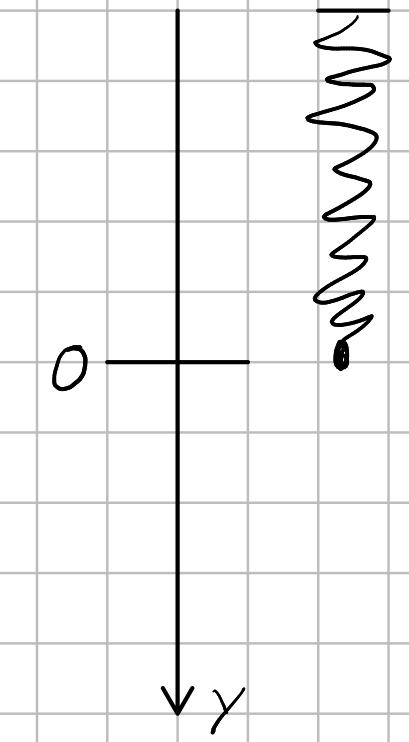
\includegraphics[keepaspectratio, width=.35\textwidth]{federpendel}
        \caption{Skizze des Federpendels}
    \end{figure}
    $y'' = -\omega_0^2y$ ungedämpftes Schwingungsmodell\\
    $\leadsto T := \frac{2\pi}{\omega_0}$ Schwingdauer\\
    \underbar{Mit Reibung}: $y''=-\alpha y' -\omega_0^2y, \quad \alpha,\omega_0>0\Leftrightarrow y''+\alpha y'+\omega_0^2y=0$
    \underbar{Mit Satz 7.4.6}:
    \[\overset{\text{charakteristisches}}{\underset{\text{Polynom}}{\leadsto}}\lambda^2+\alpha\lambda+\omega_0^2 \overset{!}{=}0,\quad \lambda_{1/2}=-\alpha\pm\sqrt{\alpha^2-\omega_0^2}\]
    \underbar{Fall 1}: $\alpha^2-\omega_0^2>0\quad\lambda_1,\lambda_2\le0$
    \[\overset{\text{Satz 7.4.6}}{\Rightarrow}y(t)=c_1e^{\lambda_1t}+c_2e^{\lambda_2t}\]
    \underbar{Fall 2}: $\alpha^2-\omega_0^2<0\quad\lambda_1,\text{ i.e. }\lambda_{1/2}=-\alpha\pm i\sqrt{\omega_0^2-\alpha^2}$
    \[\overset{7.4.6}{\Rightarrow}\text{ Lösungsraum gegeben durch }\text{span}\{e^{-\alpha t}\cos(\omega_1t),e^{-\alpha t}\sin(\omega_1t),e^{-\alpha t}\cos(-\omega_1t),e^{-\alpha t}\sin(-\omega_1t)\},\]
    i.e. $\{e^{-\alpha t}\cos(\omega_1t),e^{-\alpha t}\sin(\omega_1t)\}$ ist Fundamentalsystem
    \[\leadsto y(t)=c_1e^{-\alpha t}\cos(\omega_1t)+c_2e^{-\alpha t}\sin(\omega_1t)\]
    Bemerke: $\omega_1 < \omega_0$
    \underbar{Fall 3}: $\alpha^2-\omega_0^2=0$, i.e. $\lambda_{1/2}=-\alpha$
    \[\overset{\text{Satz 7.4.6}}{\Rightarrow}y(t)=c_1e^{-\alpha t}+c_2te^{-\alpha t}\]

    \subsection*{Existenz und Eindeutigkeit}
    \[y'(t)=f(t,y(t)),\quad y(0)=y_0 (*)\]
    $\overset{\text{Picard}}{\underset{\text{Lindelöf}}{\Rightarrow}}$ Eindeutige Lösbarkeit von $(*)$ garantiert, solange $f$ Lipschitz stetig in $y$

    \underbar{Praktisch}:\\
    $\leadsto$ komplizierte Differentialgleichungen lassen sich nicht immer analytisch lösen\\
    $\leadsto$ Numerik liebt Approximation

    \subsection*{Kleiner Ausblick: G12.3(b) (Mathe Gruppenübung)}
    \[y'(t)=\underbrace{t^2y(t)^2}_{f(t,y(t))}\text{ auf }t\in[-1,1]\text{ mit }y(0)=0\]

    \subsubsection*{Lipschitz-Stetigkeit von $f(t,\cdot)$ (global)}
    im Grunde gleichbedeutend mit $|\partial_yf(t,y)| < L\ \forall y\in\mathbb{R}$

    \underbar{Tatsächlich}: Das Existenz- und Eindeutigkeitsintervall hängt von $f$ und der optimalen Lipschitzkonstante ab
    \begin{anmerkung}
        Dies wurde angeführt, da der Satz von Picard-Lindelöf im Skript offenbar unzureichend ist, es gibt offenbar bessere Formulierungen davon.
    \end{anmerkung}
    \underbar{Bsp}: $y'(t)=3\sqrt[3]{y(t)^2},\quad y(0)=0$\\
    Lösung für $t\in[0,\infty)$?
    \[y_c(t)=\begin{cases}
            0       & ,t<c    \\
            (t-c)^3 & ,t\ge c
        \end{cases}\text{ ist Lösung für alle }c>0\]
    \[y_c'(t)=\begin{cases}
            0        & ,t<c    \\
            3(t-c)^2 & ,t\ge c
        \end{cases}\]
    \[3\sqrt[3]{y(t^2)}=\begin{cases}
            0        & ,t<c    \\
            3(t-c)^2 & ,t\ge c
        \end{cases}\]
    \begin{align*}
        f(y)  & =3\sqrt[3]{y^2}=3y^{\frac{2}{3}}       \\
        f'(y) & =2y^{-\frac{1}{3}}=\frac{2}{\sqrt[3]y}
    \end{align*}
    \begin{anmerkung}
        Lipschitz-Stetigkeit bedeutet im Grunde genommen nur, dass Abelitung beschränkt ist.
    \end{anmerkung}
    \[|f(t_1,y_1)-f(t_1,y_2|\le L|y_1-y_2|\]
    \[y'=f(y)\overset{\frac{d}{dx}}{\leadsto}y''=y'f'(y)=f(y)f'(y)\]
    \begin{anmerkungen}
        Dies alles ist wahrscheinlich eher weniger klausurrelevant, aber interessant.\\
        Die Betragsfunktion ist Lipschitz-stetig, da die Ableitung fast überall existiert und konstant (also beschränkt) ist.\\
        Wenn eine Funktion nicht stetig ist, kann sie auch nicht Lipschitz-stetig sein.
    \end{anmerkungen}
\end{document}
